\graphicspath{{figures/chapter1/}}
% Header
\renewcommand\evenpagerightmark{{\scshape\small Introduction}}
\renewcommand\oddpageleftmark{{\scshape\small Chapter 1}}

%\renewcommand{\bibname}{References}

\hyphenation{}

\chapter[Introduction]%
{Introduction}
\label{ch1}

%\begin{flushright}
%\begin{quotation}
%\textit{In order for the wheel to turn, for life to be lived, impurities are needed, and the impurities of impurities in the soil, too, as is known, if it is to be fertile.} -- Primo Levi --
%\end{quotation}
%\end{flushright}
%\npar
Catalysis, from Ancient Greek $\kappa\alpha\tau\acute{\alpha}$ (kat\'a = ``down'') and $\lambda\acute{\upsilon}\omega$ (l\'u\=o = ``loosen''), is at the heart of almost every industrially relevant chemical process. A catalyst intervenes in the reaction, allowing chemical species to come in contact and react with a specific mechanism, without being consumed. Outstanding catalysts do not only increase the rate of a given reaction, enabling processes that would not happen spontaneously, but can even be selective towards specific end products. Catalysts can be divided in homogeneous and heterogeneous, according to the phase where they are located with respect to the reactants. Homogeneous catalysts share the same phase with the reactants, and can be for instance molecules dissolved in a solvent, such as with organometallic compounds. These type of catalysts are used in many industrial processes, but have the drawback of being difficult to separate from the products, and in many cases separation is the most costly step in the catalytic cycle. For instance, in the case of biodiesel production, the recovery and purification of the products accounts for 60-80\% of the whole cost\cite{atadashi2011biodiesel}.
\npar
Heterogeneous catalysts, on the other hand, are located in a different phase with respect to the reactants, and for this reason they have the advantage of being easily separable from the reaction products. Especially green chemistry can widely benefit from heterogeneous catalysts, lowering the production costs and providing a viable alternative to petroleum \cite{chouhan2011modern}. Even if the name heterogeneous does not refer to a specific phase, industrially relevant heterogeneous catalysts are often in the solid phase. In order to exert their function, these materials must possess specific active sites that are easy to reach for the reactants, where these can adsorb, react, desorb, and ultimately diffuse back in the bulk to leave space for a new cycle. For these processes to occur, the number of active sites and the area of contact between the two phases (or surface area) must be sufficiently high, and reactants and products must be able to easily diffuse in the material. 
\npar
All the above mentioned properties can be found in nanoporous materials, which possess pores with a diameter of $<$ 100 nm, and and are extensively used in the field of heterogeneous catalysis. According to the classification by the International Union of Pure and Applied Chemistry (IUPAC) \cite{mcnaught1997compendium}, nanoporous materials can be differentiated on the basis of their pore size into microporous (pore size $<$ 2 nm), mesoporous (pore size between 2 and 50 nm) and macroporous (pore size $>$ 50 nm). Their pore structure provides them with an exceptionally high surface area, that for some materials can reach values larger than 7000 m$^2$/g \cite{farha2012metal, honicke2018balancing}. This facilitates diffusion of reactants inside the material, and allows shape selectivity to give specific products. Well-known classes of nanoporous materials include zeolites and metal organic frameworks (MOFs) \cite{liang2017heterogeneous}. Zeolites were one of first heterogeneous catalysts to be industrially exploited, and are the workhorses of petrochemistry, among other applications. They are extremely robust due to their inorganic nature and can withstand harsh reaction conditions. In contrast, MOFs are novel hybrid materials that are less robust, but extremely versatile. They possess even higher porosity, diverse composition, high metal content and tunable organic functions, and for these reasons they have a high catalytic potential. 
\npar
In general, the study of solid heterogeneous catalysts is not trivial, as the exact concentration and nature of the active sites is often unknown. It is not always clear, in fact, where exactly the active sites may be located in the material, and how they interact with molecules. Moreover, these materials are far from perfect, and are often the defects which are tremendously important to induce the catalytic properties. In this sense, molecular modeling offers a complementary platform, not only to understand the catalytic function, but also to determine structure--activity relationships and to design structures to target specific applications\cite{van2015advances}. 
%This is especially important in the study of MOFs.
%The steady progress of industrial chemistry is tightly connected to the discovery of novel materials that can target specific applications. In this context, hybrid materials, such as MOFs represent a growing research field, where new applications are being explored.

\begin{figure}[!htbp]
	\centering
 	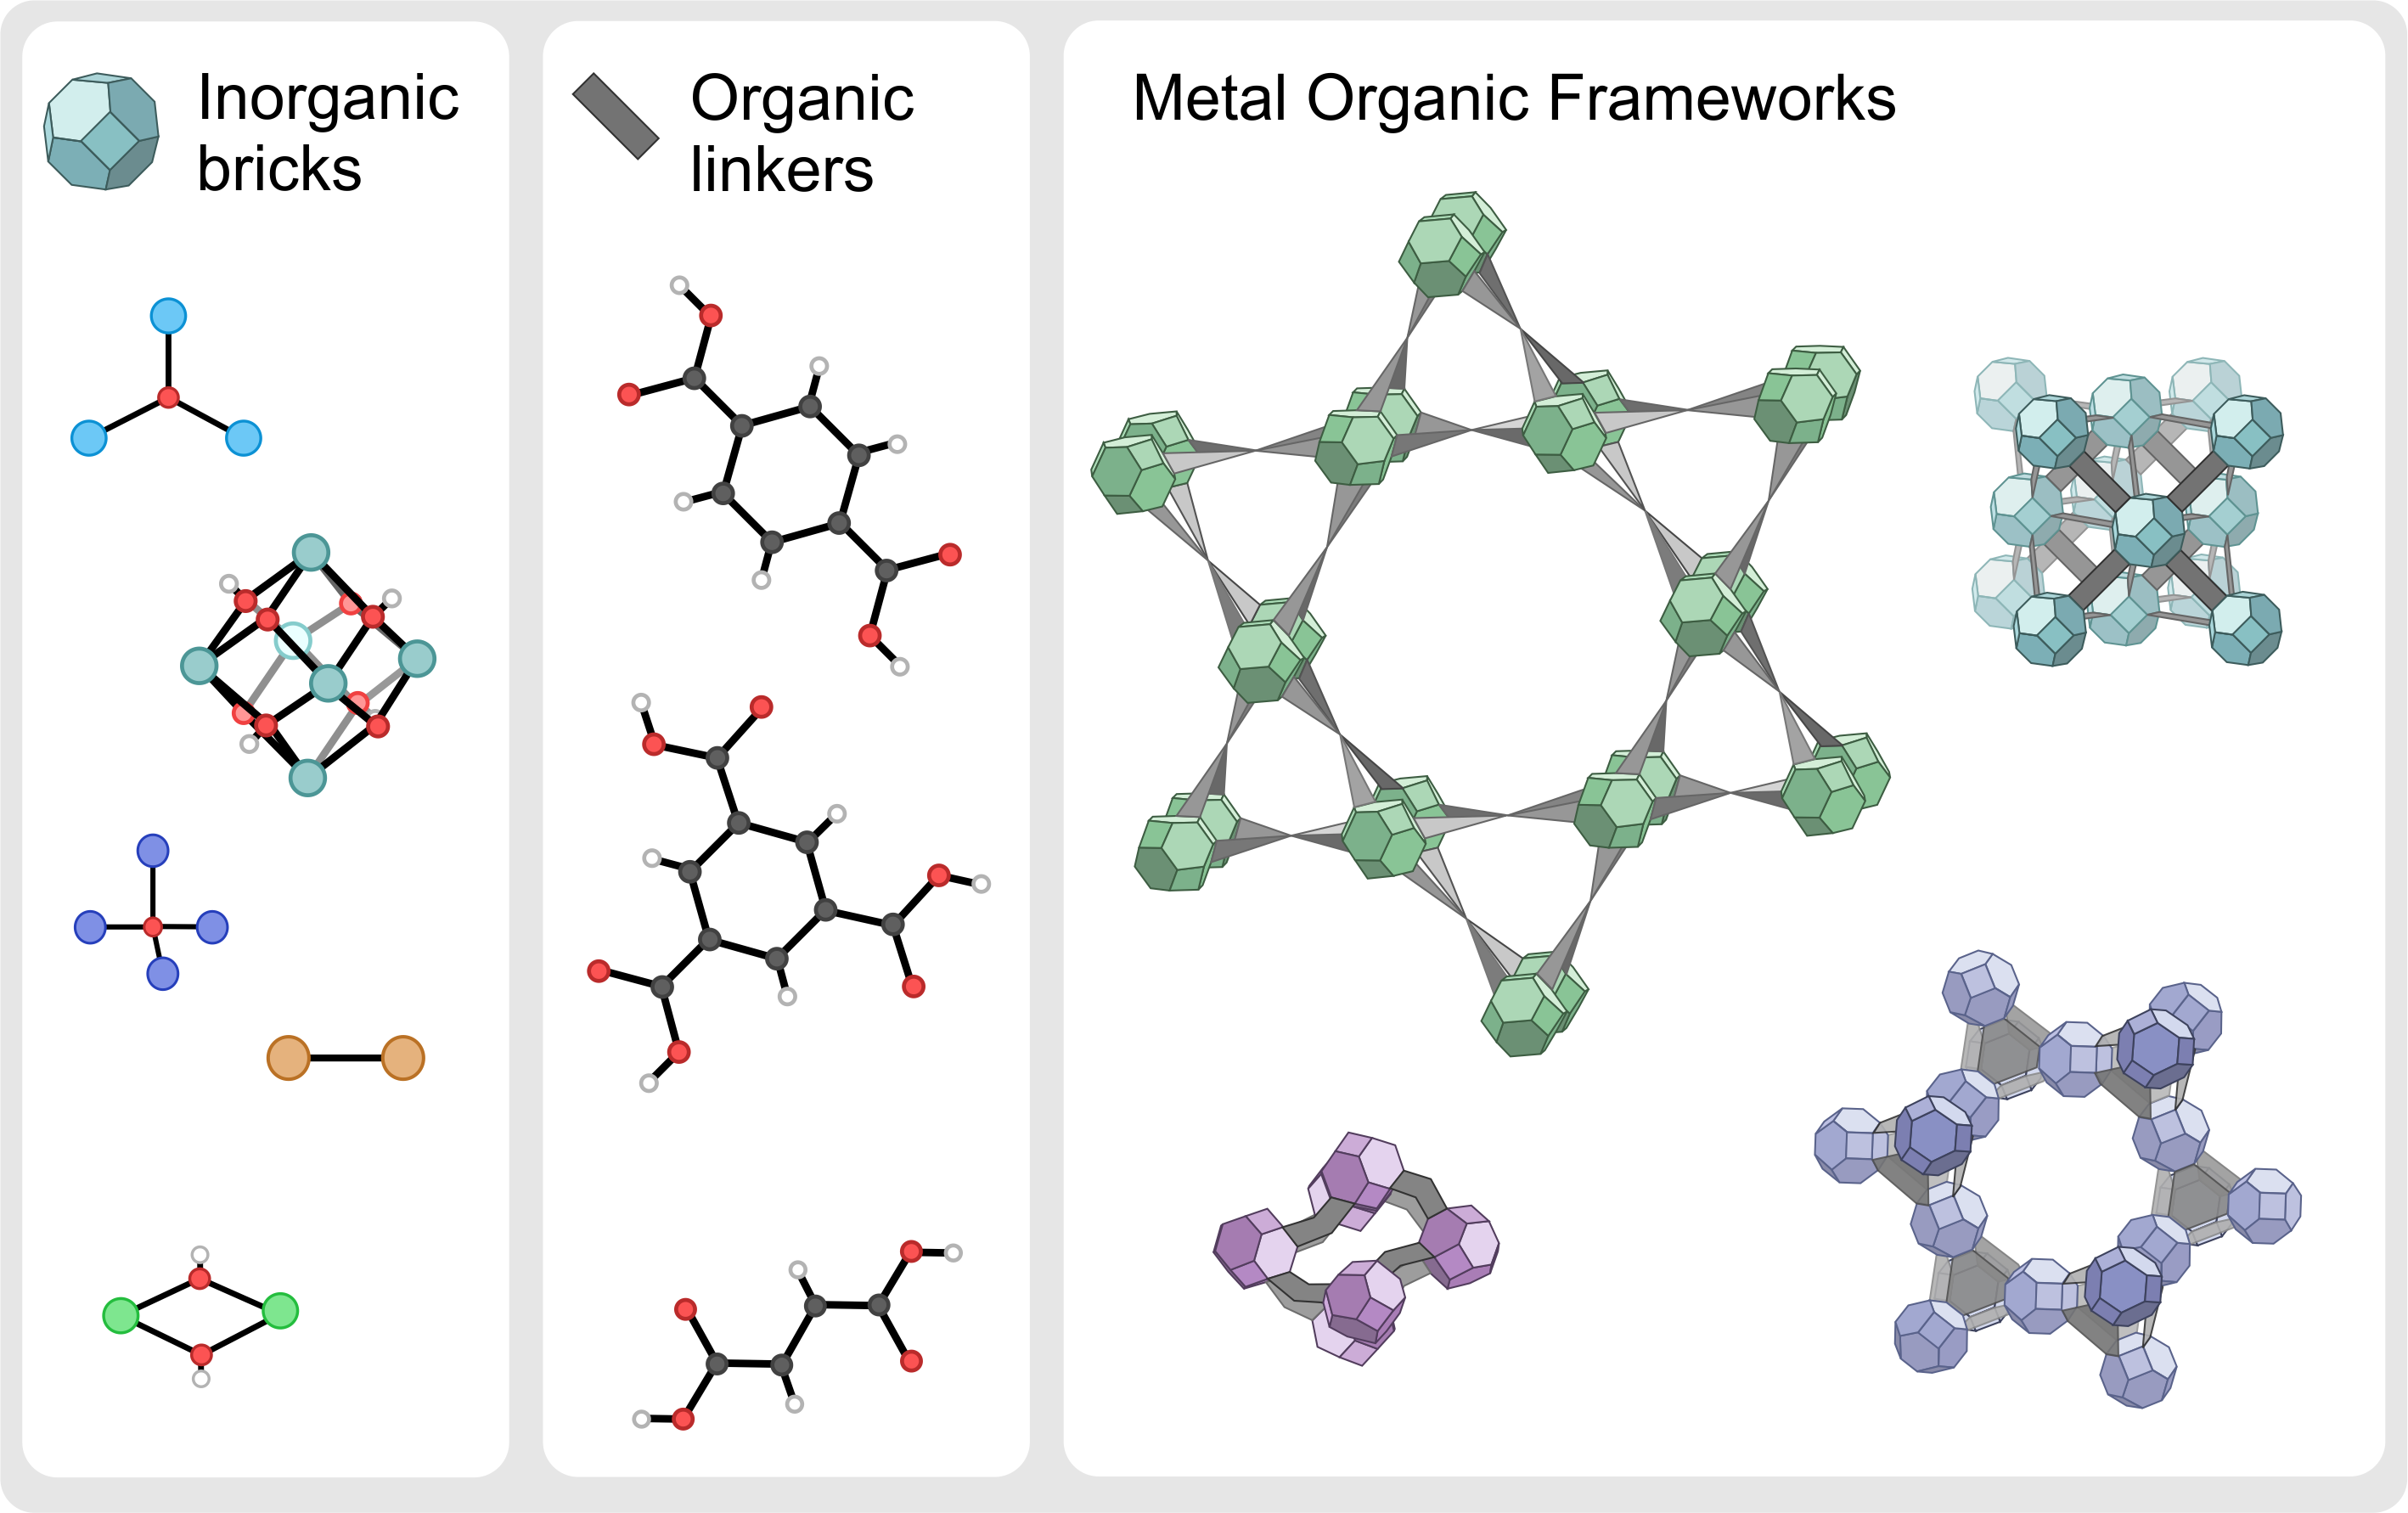
\includegraphics[width=1.0\textwidth]{MOFs}
	\caption{Schematic representation of the building block design in Metal-Organic Frameworks (MOFs). Left panel: some examples of inorganic bricks; middle panel: some examples of organic linkers; right panel: some MOFs with different topologies, pore size and shape}
	\label{fig:MOFs}
\end{figure}

\section{Metal Organic Frameworks}
MOFs are one of the most intriguing class of materials of current science. These materials, first called 'porous coordination polymers' (PCPs) were discovered in the late 50's, but only at the end of the past century with the works of Robson\cite{batten1995two,hoskins1990design}, Kitagawa\cite{kitagawa1991synthesis, kitagawa1993synthesis}, Yaghi\cite{yaghi1995hydrothermal} and F\'{e}rey\cite{riou1998hybrid}, the scientific community started to understand their full potential. At first the main focus of MOF research was in the discovery of new structures. However, in the last few decades, the field has seen an incredible explosion in scientific and industrial interest, with new applications being continuously explored\cite{furukawa2013chemistry}. MOFs are hybrid nanoporous materials that are composed by metal or metal--oxo clusters connected by multitopic organic linkers, to form multidimensional porous structures. Compared to the already well--known zeolites, MOFs can be constructed without templating agents, with a far greater number of metals and with an exceptional structural diversity. In fact, their particular building block design (Figure \ref{fig:MOFs}), that makes use of secondary building units (SBUs), allows the creation of an almost infinite number of crystalline structures with different topology and chemical composition. 
\npar
The coordination bonds which lie at the basis of MOF structures are weaker than in other heterogeneous catalyst such as zeolites. This on the one hand makes them less robust, but on the other allows facile structural modifications which are impossible to do on zeolites. In principle, the nature of the SBUs and their association can be finetuned\cite{stock2011synthesis}, allowing control of properties such as pore shape and size, functionalization, or surface area. The response to chemical and physical stimuli can this way be easily modulated \cite{zhou2014metal,zhou2012introduction}. 
One of the most intriguing concepts is the isoreticular synthesis, by which inorganic or organic SBUs can be replaced by topologically identical (or similar) building blocks. This way, starting from a given MOF precursor, whole families of MOF materials can be synthesized spanning a range of pore size and functionality. For instance, the pore size can be significantly increased up to the mesoporous range by using longer isoreticular linkers, such as in the IRMOF series, based on the MOF--5 precursor \cite{eddaoudi2002systematic}. 
\npar
The tunability of MOF structures, along with their high crystallinity, metal content and porosity, are very appealing for application in different industrially relevant fields, such as catalysis, gas storage and separation, drug delivery or sensing, as displayed in Figure \ref{fig:mof-applications}. More specific applications are being further explored, such as warfare agents decomposition, magnetic applications, or membrane separation \cite{furukawa2013chemistry}. At present moment, the main limitation for large scale application lies in the structural stability. 
%
%
\begin{figure}[htbp]
	\centering
 	\includegraphics[width=1.0\textwidth]{mof-applications}
	\caption{Schematic representation of some of the numerous MOF applications.}
	\label{fig:mof-applications}
\end{figure}
%
\npar
The study of MOFs has seen a continuous evolution in the past decades.
Following the nomenclature proposed by Kitagawa, we can differentiate between three generations of MOFs\cite{kitagawa1998functional}. First generation MOFs are defined as having a guest--molecules supported pore system that collapses when these are evacuated. For this reason, this first generation of MOFs found very limited use for practical applications. Those of second generation are more robust and have permanent porosity, that is retained even in absence of guest molecules. These materials show high potential for catalysis and other applications and are the main object of this dissertation. Finally, third generation MOFs are characterized by flexible pores that can reversibly change shape with the presence of guest molecules, or upon certain stimuli, such as temperature or pressure. Matsuka \textit{et al.}\cite{matsuda2004guest} identified five types of response mechanisms in MOFs, denoted as shrinking, expanding, reshaping, swelling and gate opening or closing. A perspective on the types of stimuli that can induce responsive in MOFs has been reported in the work of Coudert \cite{coudert2015responsive}.

\subsection*{Defects and active sites}
MOFs are crystalline materials that possess structural disorder, such as vacancies. If at first this was seen as a drawback, limiting stability, it has been accepted that they can play a key role in the performance of the material. Defect--containing MOFs and defect engineering have become an active field in MOF research, representing an additional way to finetune and enhance the material properties. 
Following the classification proposed by Sholl \textit{et al.} \cite{sholl2015defects}, defective sites in MOFs can be either point vacancies (such as missing linkers or clusters) or extended ones. Fang \textit{et al.} \cite{fang2015defect} further divided extended defects into dislocations, planar defects, and micro-- and mesoscale volume defects. 
\npar
At low defect concentration, a random distribution of isolated point defects can be found, whereas at higher concentrations, clustering could occur\cite{cliffe2014correlated} if the presence of a vacancy is influenced by other vacancies in proximity. The complexity arising from structural disorder makes the study of defects a current challenge in MOF research. In order to control their effect on certain properties, it is important to have precise information on their location, type and dispersion. Common experimental strategies for the characterization of defects in MOFs involve electron and fluorescence microscopy, Raman, infrared and X-ray spectroscopy, power and single--crystal X-ray diffraction\cite{fang2015defect}. Complementary to experiment, molecular modeling provides an important tool to obtain atomic scale resolution on the defect sites and understand how they impact specific properties.
\npar
Particularly for catalysis and adsorption, vacancies in the material lead to two main effects: 1) an increase in porosity and mass transport, and 2) the presence of undercoordinated metal atoms, introducing highly desired Lewis acid sites. 
%\subsection*{MOFs as single site catalysts}
In this sense, provided the structures are stable at reaction conditions (i.e. no leaking is observed), 
MOFs are true single--site heterogeneous catalysts, that contain well--defined active sites which are inherent part of the framework\cite{yang2019catalysis}. We particularly refer to the importance of catalysis in MOF research, shown by the number of publications on the topic (Figure \ref{fig:citation_report}). According to the classification proposed by Rogge \textit{et al.} \cite{rogge2017metal}, we can distinguish between three types of single--site catalysts in nanoporous materials, in which active sites for catalysis can arise from coordinatively unsaturated metals (type I), metal atoms embedded in porphyrin--based ligands (type II) or reactive functional groups (type III). 
\npar
Coordinatively unsaturated metals are are Lewis acid sites that can be present in the framework such as in HKUST--1\cite{chui1999chemically}, or can be introduced by intentional creation of defects, such as in the stable UiO--66 MOF \cite{vandichel2015active}. Another procedure that can lead to open metal sites without generating vacancies is the dehydration upon thermal treatment. To date, a plethora of MOFs have been synthesized containing open metal sites that possess different Lewis acidity. Moreover, their acidic properties can further be tuned by functionalization of linkers and bricks. This way, it is in principle possible to engineer a material for a target catalytic application.

\begin{figure}[!htbp]
	\centering
 	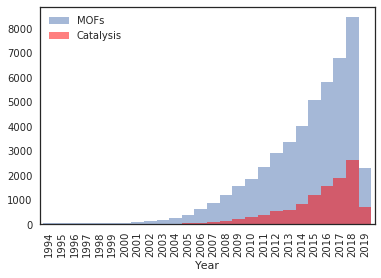
\includegraphics[width=0.8\textwidth]{citation_report}
	\caption{Number of publications on MOFs and catalysis in MOFs in years 1985-2018, showing the importance of catalysis in MOFs as indicated by Web of Science}
	\label{fig:citation_report}
\end{figure}
%
\subsection*{Post--synthetic modification}
When it is not possible to introduce functionalities with direct synthesis, post--synthetic modification (PSM) \cite{wang2009postsynthetic, cohen2011postsynthetic} has become a well established procedure that allows the preparation of MOF materials with specific chemical composition. Via this technique, it is possible to modify the crystal after the synthesis, allowing to finetune the properties of the material. Moreover, multi--functional sites can be integrated at the same time in the crystals \cite{li2016applications}. PSM strategies include encapsulation of guest molecules or nanoparticles in the pores, modifications of the linkers without breaking the metal--ligand bond, or post synthetic exchange (PSE) of linkers and metals, where building blocks are dynamically exchanged. PSE can also involve terminal ligands, or modulators, that do not contribute in connecting different bricks. This way, building blocks can be exchanged in a dynamic way. Moreover, they can also be eliminated from the framework to create vacancies, provided the material retains its crystallinity. For this reason, PSM has been used as an efficient strategy to introduce defective sites in MOFs. As one may expect, sufficient structural stability under the PSM conditions is a necessary prerequisite in order to apply PSM techniques \cite{garibay2010isoreticular}.
%
\subsection*{Stability}
In general, to function at operating conditions and to withstand modifications, materials need to retain their mechanical, thermal and chemical stability at those conditions\cite{howarth2016chemical}. For instance, mechanical stability is needed when compressing MOF in pellets or other shapes for industrial processes\cite{chapman2009pressure}. Catalysis often also requires thermal stability, as the materials must be able to resist harsher conditions for certain processes such as in petrochemistry. Finally, chemical stability is crucial for many applications, such as drug delivery, molecular separation, or catalysis\cite{horcajada2010porous}. 
\npar
Unfortunately, the M--L coordination bond that makes MOFs so tunable is also regarded as one of their main drawbacks\cite{keskin2010can, canivet2014water, kizzie2011effect}, as it is responsible for the lower structural stability when compared to already established nanoporous catalysts such as zeolites. 
%For this reason, MOF research has focused on the development of stable materials. 
For example, the first synthesized MOFs such as \ce{Cu2+} trimesate HKUST-1, or MOF-5, composed by \ce{Zn2+} clusters and BDC linkers were degraded by water even at mild conditions\cite{greathouse2006interaction, low2009virtual, kaye2007impact, decoste2013effect}. Moreover, mechanical, thermal and chemical stabilities can further decrease in the presence of defects. Very few MOFs show stability towards water and at different pH conditions\cite{leus2016systematic}, in particular the family of Zr--based MOFs. 

\subsection*{Zr--based MOFs}
Recently, a class of outstandingly robust MOFs have been synthesized \cite{furukawa2014water}. Zr--based MOFs\cite{bai2016zr} which exploit the robustness of the Zr--O bond, show an unprecedented stability and are at present time one of the most studied classes of MOFs (Figure \ref{fig:Zr-MOFs}). Moreover, zirconium is an ubiquitous metal that is present in biological systems and has low toxicity, as well as limited cost. This makes Zr--based MOFs particularly promising for applications in catalysis, gas sorption, and drug delivery. An overview of the plethora of possible structures that can be synthesized with different inorganic SBUs can be found in a recent review by Bai \textit{et al.} \cite{bai2016zr}.
\npar
%%
\begin{figure}[!htbp]
	\centering
 	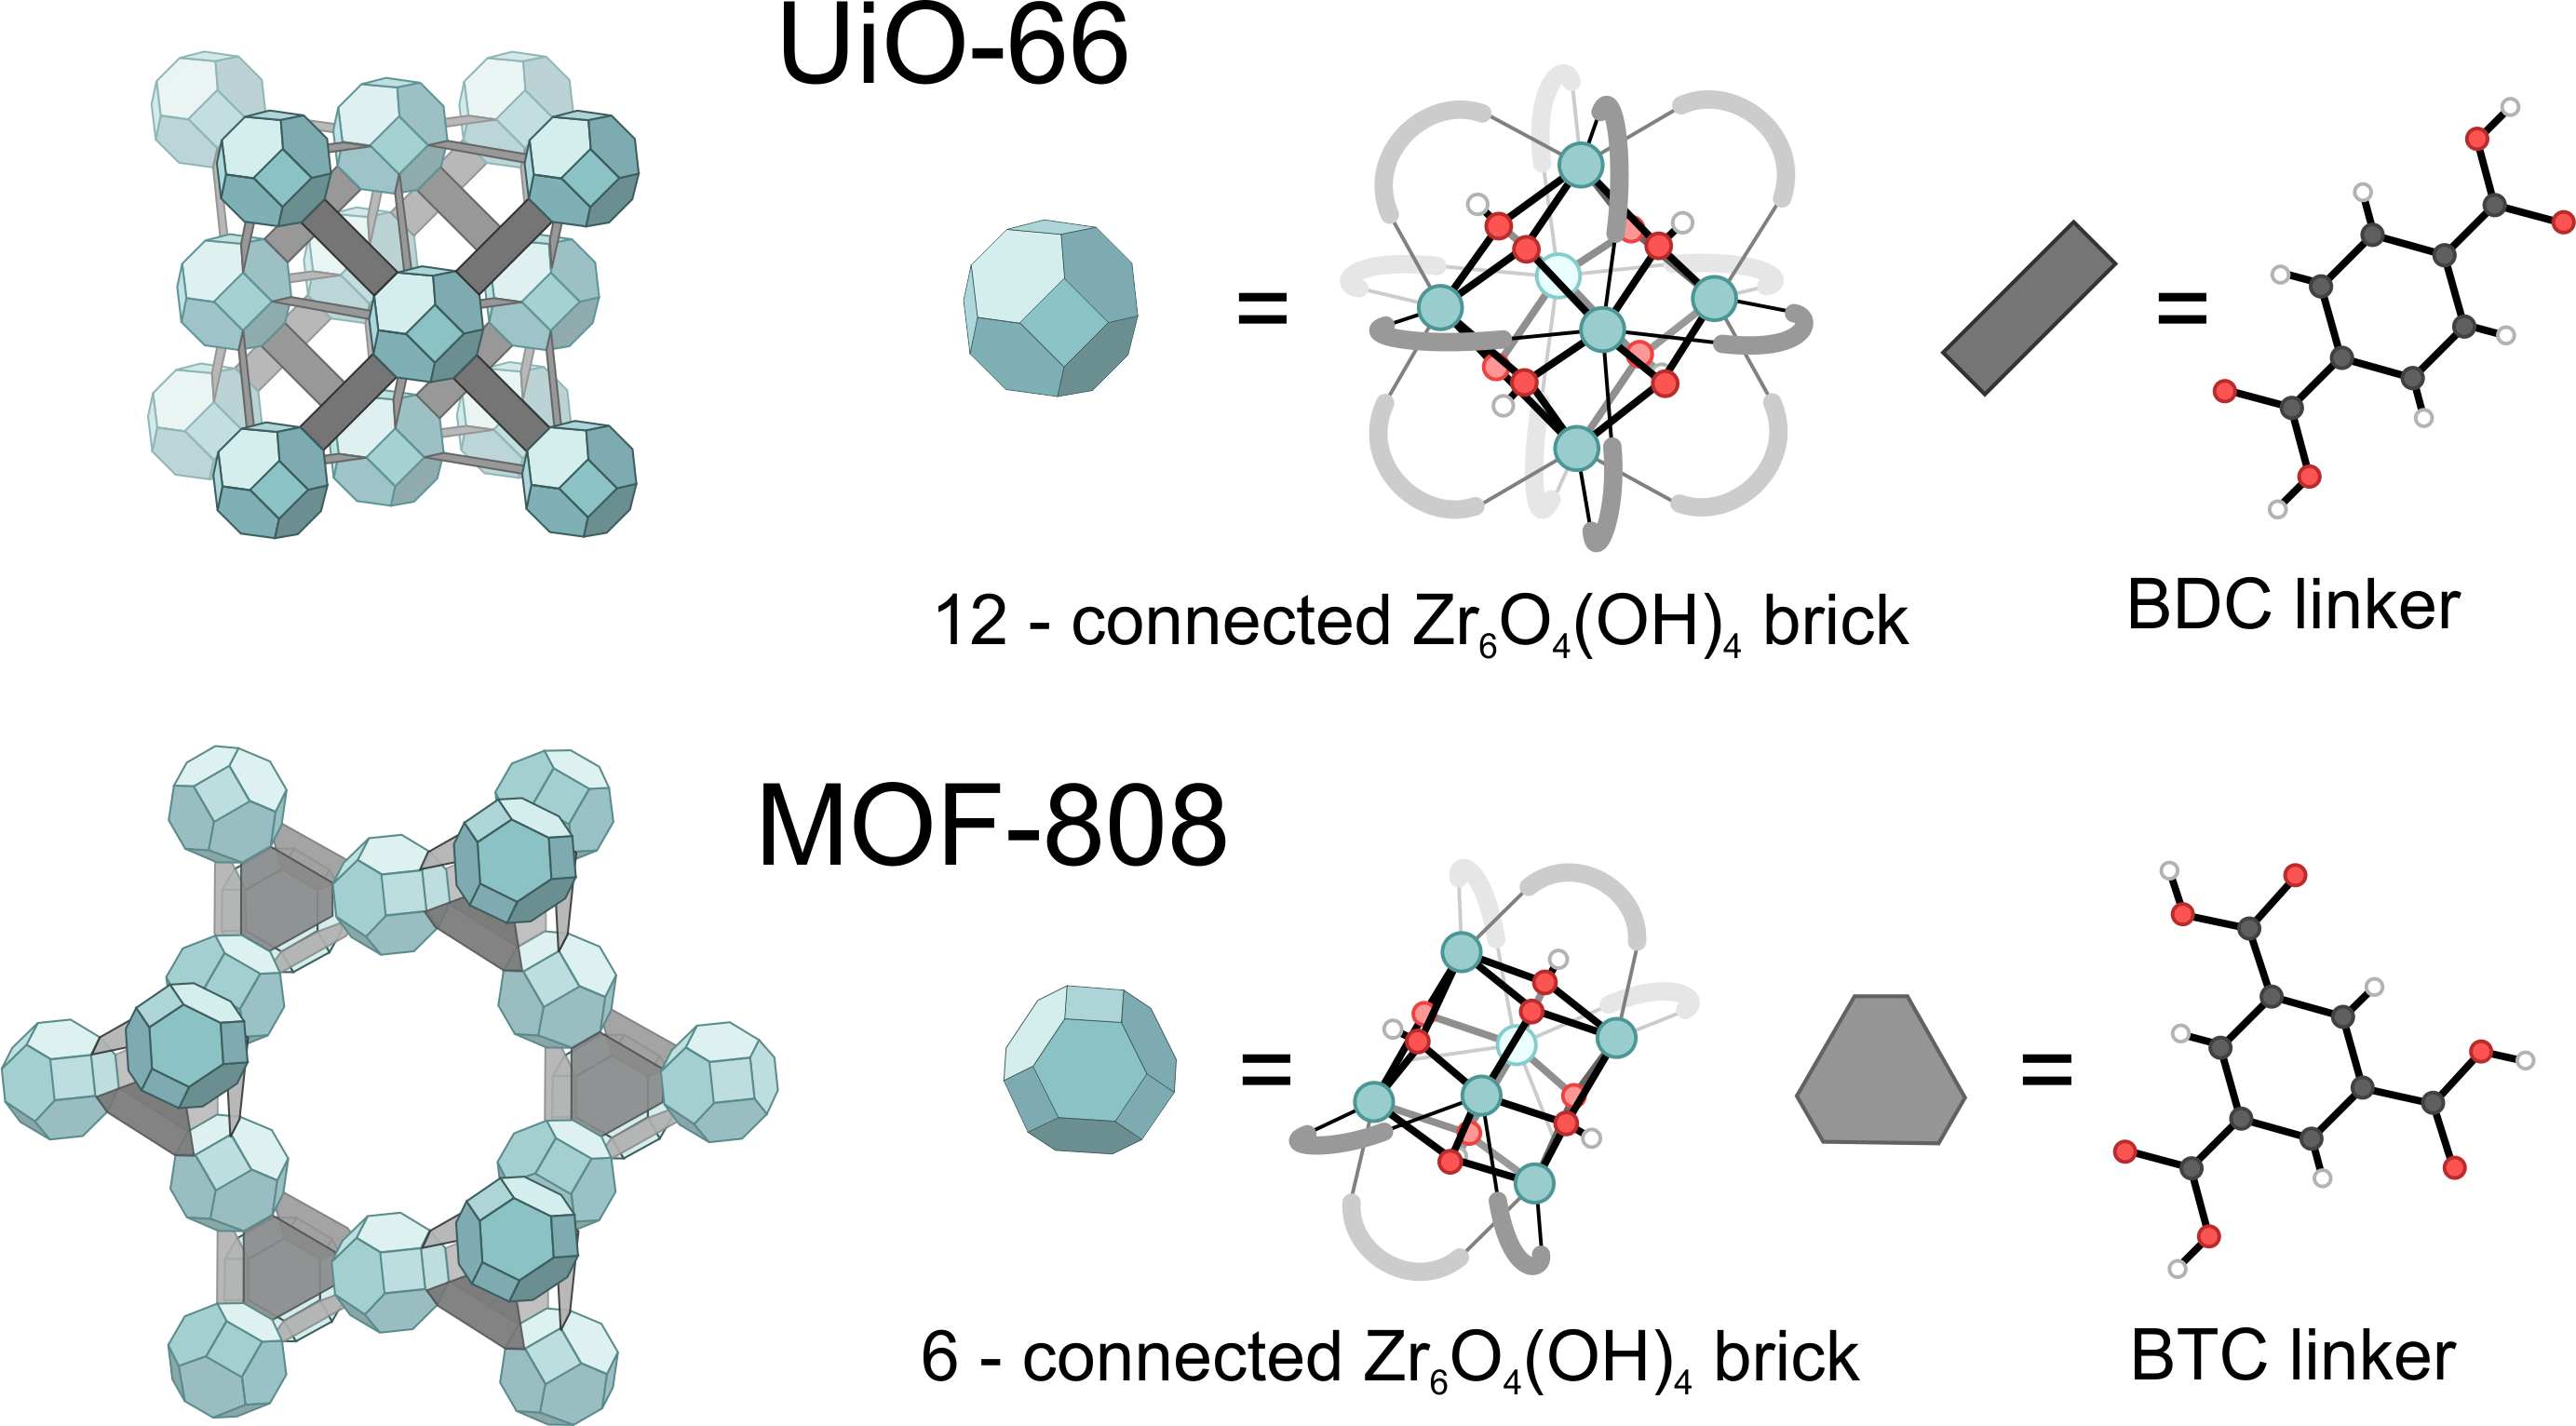
\includegraphics[width=1.0\textwidth]{Zr-MOFs}
	\caption{Structure of UiO--66 (top) and MOF--808 (bottom), the two Zr--MOFs investigated in this work of thesis.}
	\label{fig:Zr-MOFs}
\end{figure}
%%
The vast majority of these materials is characterized by Zr(IV) atoms in a high coordination state (Figure \ref{fig:Zr-MOFs}), which interact strongly with the oxygens of carboxylate linkers of various topology. These MOFs are characterized by a \ce{Zr6O4(OH)4} cluster in which each of the 6 zirconium atoms is connected to 4 oxygen atoms (two $\mu_3$--OH and two $\mu_3$--O), each of which is in turn connected to three zirconium atoms, forming a polyhedron. Each zirconium atom can form 4 other bonds with ligands, accommodating up to 24 metal--ligand bonds per cluster. Every zirconium atom can therefore form a total of 8 coordination bonds oriented in a square--antiprismatic geometry, yielding a rich range of possible structures that can be synthesized with connectivity ranging from 12, as in UiO--66\cite{cavka2008new}, to 6 which is found in MOF--808\cite{furukawa2014water} (see Figure \ref{fig:Zr-MOFs}). The dual Lewis acid/base nature of the Zr--carboxylate bonds, along with the high metal oxidation state, gives rise to strong interactions between the SBUs, thus allowing processes such as PSM without compromising the stability of the structures. The high degree of connectivity between inorganic and organic SBUs lies at the origin of the high structural stability found in Zr--based MOFs\cite{bai2016zr, leus2016systematic}. Open metal sites in these materials can be present if the brick connectivity is lower than 12. This can be an inherent property of the structure, such as in the 8--fold connected NU--1000 \cite{mondloch2013vapor}, or can be induced by introduction of structural defects. Zirconium atoms that remain undercoordinated are Lewis acid sites where reactants can adsorb and that can function as catalytic centers.

\subsection*{UiO--66}
The first material belonging to this class of Zr--based MOFs is the Zr--therephtalate based UiO--66, and was first synthesized at the Universiteit i Oslo (UiO) by Lillerud and coworkers\cite{cavka2008new}. The UiO-66 material, shown in Figure \ref{fig:Zr-MOFs} (top), is one of the most studied MOFs thus far and was an inspiration of other MOFs within this family. UiO--66 is characterized by an extremely high connectivity that gives rise to an exceptional structural stability. In this material, each \ce{Zr6} SBU is connected to 12 therephthalate (or benzenedicarboxylate (BDC)) linkers forming a cubic close packed structure with a space group F\={m}3m, No. 225. In this structure there are two different cavities of octahedral and tetrahedral shape, with window sizes of 10 \AA\ and 25 \AA, respectively. Each octahedral cage shares triangular windows with eight tetrahedral cages. 
This results in an extremely robust material which is stable up to 648 K and in a broad range of protic and aprotic solvents and pH conditions. Moreover, the \ce{Zr6O4(OH)4} bricks can be reversibly dehydrated upon thermal treatment at temperatures between 523 and 573 K. Up to two water molecules can be formed this way, yielding a \ce{Zr6O6} brick, where the zirconium atoms have a coordination of 7\cite{valenzano2011disclosing}. Lowering of zirconium coordination by dehydration can be a strategy to create open metal sites, along with the creation of defects.
\npar
A whole family of isoreticular MOFs can be derived from UiO--66 by using linkers of different size, spanning from fumaric acid\cite{wissmann2012modulated} up to terphenyldicarboxylic acid\cite{schaate2011modulated}, allowing to significantly tune pore size and surface area. Interpenetrated MOFs with UiO--66 topology have been also reported if longer linkers are used\cite{schaate2011porous}, however with a decrease in surface area. Moreover, different functional groups can be appended to the phenyl rings, such as bromo, amino, nitro, or naphthalene. Garibay and Cohen showed that UiO--66--\ce{NH2} can be further modified to yield new functionalized frameworks \cite{garibay2010isoreticular}. Also the inorganic SBUs can be modified, for instance introducing titanium or hafnium\cite{kim2012postsynthetic}. Moreover, PSM can lead to creation of defects and open metal sites, as will be shown in \textbf{PAPER IV}. The exceptional thermal and chemical stability of UiO--66, along with its high connectivity, allows all these modifications of the structure, and for this reason, this material is often considered as a perfect MOF archetype, where new techniques can be tested. 

\subsubsection*{Defects on UiO-66}
%chap 11 of book from Garcia
%The perfect crystalline UiO--66 structure, where every zirconium atom is 8--fold coordinated, does not possess open metal sites for catalysis. 
The high connectivity of the UiO--66 material allows the presence of structural vacancies. It has been generally accepted that the material can contain defects in the form of missing linkers or clusters (Figure \ref{fig:defectiveuio}). These defects naturally originate during synthesis, as shown by experimental results, such as symmetry--forbidden reflections in the PXRD pattern, metal--linker ratio obtained by thermogravimetric analysis (TGA), higher than expected surface area, appearance of O--H stretching bands in the FTIR spectrum etc. \cite{shearer2014tuned, valenzano2011disclosing}. Moreover, it was later discovered that the number of defective sites can easily be tuned by adapting the synthesis conditions, such as temperature and type of modulator\cite{wu2013unusual, shearer2016defect}.
\begin{figure}[!hbtp]
	\centering
 	\includegraphics[width=1.0\textwidth]{defectiveuio}
	\caption{Representation of the UiO--66 material with missing linkers and clusters displayed in red. In this dissertation, we mainly focus on missing linkers.}
	\label{fig:defectiveuio}
\end{figure}
\npar
Defects can influence the material properties to a large extent. The beneficial role of defects in UiO--66 has been explored in many applications such as gas storage and separation\cite{wu2013unusual, ren2014modulated}, sensing\cite{stassen2016towards}, drug delivery\cite{cunha2013rationale} and catalysis\cite{vermoortele2013synthesis, rogge2017metal}. The physical properties of defective UiO--66 differ according to the number of defects and their location, as has been extensively studied both theoretically and experimentally \cite{rogge2016thermodynamic, devos2017missing, cliffe2014correlated, borges2016proton}. A decrease in the connectivity in the structure will naturally lead to a decrease in stability of the material. However, the extremely high connectivity of UiO--66 allows the presence of both missing linkers and clusters without loss of crystallinity. In this context, Rogge \textit{et al}. investigated the influence of all possible configurations of one to two linker vacancies on the stability of UiO-66. The equilibrium volume is not affected by such vacancies, however properties such as bulk modulus and loss--of--crystallinity pressure, which in turn influence the stability, are affected by the number and configuration of missing linkers \cite{rogge2016thermodynamic}. 
De Vos \textit{et al}.\cite{devos2017missing} investigated the electronic properties for all possible configuration of defective UiO--66 with up to three missing linkers, showing that some configurations are energetically more stable than others, and that the number and position of missing linkers affect the band gap of the material. From these studies performed on small unit cells, it is already clear that the number of possible defective configurations can be extremely high, and it is still unclear to what extent such point defects are disordered in the material. A regular distribution of point defects that involve missing clusters can lead to different phases in the material, from \textit{fcu} (non-defective), to \textit{bcu} (missing linkers with open channels), \textit{reo} (missing clusters) to \textit{scu} (missing linkers and missing clusters). Missing clusters could in principle increase the catalytic activity of the material more than missing linkers due to the larger pore size. Recently, Cliffe \textit{et al}. \cite{cliffe2014correlated} showed in a combined theoretical-experimental work that missing clusters on UiO-66(Hf) were correlated and formed nanodomains in the material, characterized by a \textit{reo} phase. The presence of missing clusters or missing linkers can be affected by the choice of modulator\cite{svane2018vacancy}. These reports shed light into the complex nature of defects in nanoporous materials. 

\subsubsection*{Active sites for catalysis in UiO--66}
One of the breakthroughs of MOF research was the discovery that UiO--66 could contain a high number of open metal sites. As reported earlier, active sites for catalysis in UiO--66 and other Zr--MOFs are present when the zirconium connectivity is decreased from its equilibrium value of 8.
\npar
%active sites by defects
A first way to obtain coordinatively unsaturated zirconium sites is by creation of defects, in the form of missing linkers or clusters. The inherent vacancies in UiO--66 bring unsaturated zirconium Lewis acid sites\cite{wu2013unusual, shearer2014tuned, vermoortele2013synthesis, vandichel2015active, liu2016probing} and at the same time enhance the accessibility of the reactants to the active sites as the pore volume increases. The synthesis of defective UiO--66 can be tuned via modulators such as formic acid or trifluoroacetic acid (TFA), that are competing with BDC linkers in binding to the inorganic SBU. 
Vermoortele \textit{et al}. first showed in a dual computational--experimental study that the Lewis catalyzed cyclization of citronellal requires missing linkers\cite{vermoortele2012electronic}. For Meerwein reduction, another Lewis catalyzed reaction, the catalytic activity of UiO--66 could be significantly increased by making use of TFA, that introduced a large number of linker vacancies. Additionally, the non-modulated material that contained only a small number of defects showed nearly no catalytic activity\cite{vermoortele2013synthesis}. Such relationship between catalytic activity and amount of defects has been reported for different Lewis catalyzed reactions giving clear evidence that the catalytic centers are located on the defective sites\cite{vermoortele2012electronic, vermoortele2013synthesis}. 
\npar
The molecular characterization of the defective sites on UiO--66 has been an ongoing research interest in MOF literature. Particular focus has been given on the species adsorbed on the defective site and on the coordination environment of zirconium (Figure \ref{fig:bronsted-lewis-uio}). Early experimental work by Lillerud and coworkers \cite{oien2014detailed} reported that when linker vacancies were present, XRD characterization of the material showed two types of Zr--bonded oxygen atoms. The first type was BDC oxygen, and the other was associated to water species coordinated to the zirconium on the defect site. Later from SXRD measurements, the group of Yaghi \cite{trickett2015definitive} proposed that the two Zr--bonded oxygens belonged to physisorbed water molecules and that the charge compensating species was a hydroxyl group. However, following reports did not confirm such configuration.

\begin{figure}[!bhtp]
	\centering
 	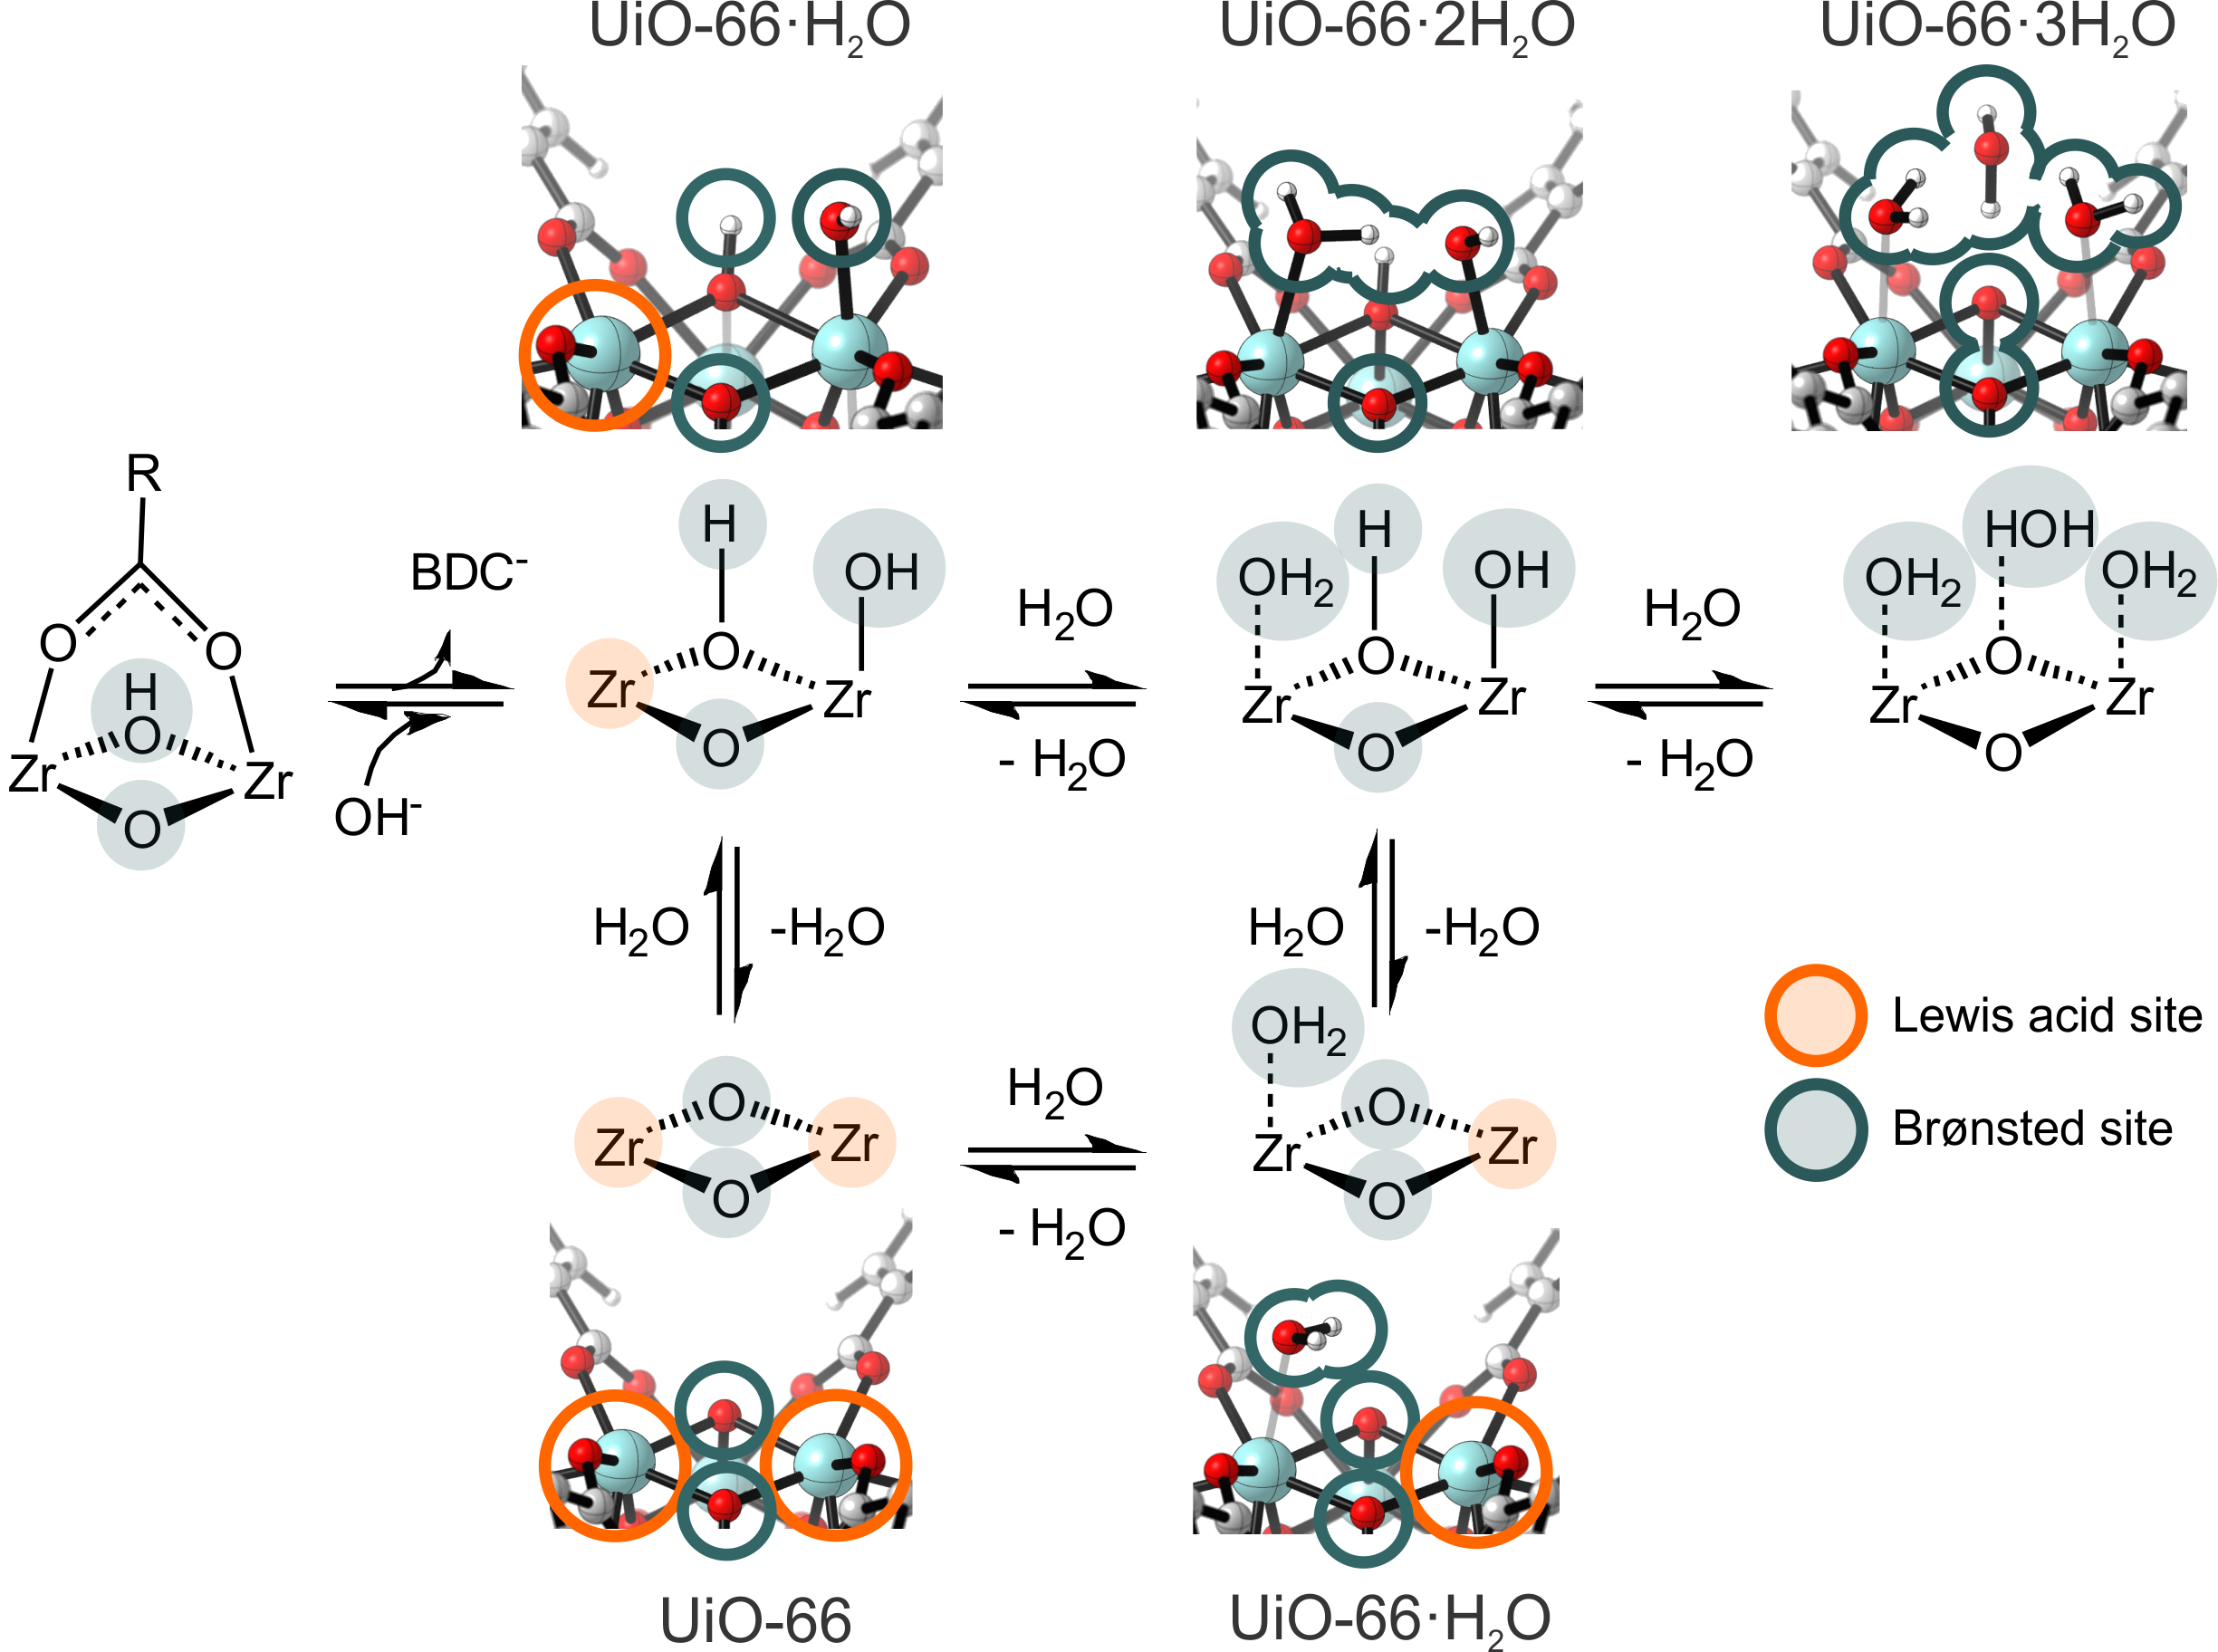
\includegraphics[width=1.0\textwidth]{bronsted-lewis-uio}
	\caption{Lewis and Br\o{}nsted sites that are created when a linker is removed from the UiO--66 zirconium brick, with different number of coordinated water molecules.}
	\label{fig:bronsted-lewis-uio}
\end{figure}
\npar
Molecular simulations were essential to shed light into the detailed molecular structure of the defective brick. Ling and Slater \cite{ling2016dynamic} performed MD simulations starting from the configuration proposed by Yaghi and showed a progressive stabilization towards another structure where the two adjacent zirconium atoms were coordinated to a physisorbed water molecule and a hydroxyl group, as shown in Figure \ref{fig:bronsted-lewis-uio}. These sites have been confirmed by a comprehensive computational study of different adsorption possibilities of up to three water molecules on defective UiO--66 performed by Vandichel \textit{et al}. \cite{vandichel2016water} and by simulations performed in this thesis.
Such water and hydroxy species are strongly interacting with the zirconium atoms and are sources of Br\o{}nsted sites, as indicated in Figure \ref{fig:bronsted-lewis-uio}. It was remarkable to discover that some catalytic processes are not catalyzed by undercoordinated Lewis acid sites, but need also Br\o{}nsted sites arising from defect--coordinating species, as will be shown in \textbf{PAPER I}. Apart from the interactions of water with the active sites, they may also have a strong influence on the proton conductivity of the material. Serre and coworkers reported that a hydrogen bonded network that spans the octahedral and tetrahedral cages is responsible for the high proton conductivity showed by UiO-66 at high temperatures \cite{borges2016proton}. Kitagawa \textit{et al.} showed the positive role of defects in proton conductivity in the UiO-66 material, as defective sites provide both larger pores and zirconium undercoordinated sites where water species are adsorbed and can function as proton donors \cite{taylor2015defect}. Farha and coworkers identified three types of acidic protons in the material by means of potentiometric titration: $\mu_{3}$--OH belonging to the inorganic SBU, and two arising from subsequent deprotonation of the physisorbed water and hydroxyl group on the defective site. They made use of the acidic protons belonging to physisorbed water for a quantification of defects in the material as alternative to TGA \cite{klet2016evaluation}. The mechanism associated to the change in topology of the hydroxyl groups on the inorganic SBU has been investigated by Yang \textit{et al}.\cite{yang2016tuning}. The interaction between defect--coordinating water molecules and zirconium atoms is strong, and UiO--66 can be partially hydrolized\cite{decoste2013stability} while retaining its stability, as will be further discussed in this dissertation.
\npar
The defect--coordinating species can be removed by thermal activation at T $>$ 423 K (more information on this process is given in \textbf{PAPER I}). The more loosely bonded physisorbed water is the first to leave the defective site, followed by the chemisorbed water. The dehydrated active site obtained this way is missing a $\mu_{3}$--OH proton and has two 7--fold coordinated zirconium open metal sites as shown in Figure \ref{fig:bronsted-lewis-uio} (bottom left). 
\npar
%active sites by dehydration
The second activation process by which open metal sites can be created on UiO--66 is the reversible dehydration of the \ce{Zr6O4(OH)4} cornestone to obtain \ce{Zr6O6} by removal of up to two water molecules performed at a temperature range between 523 and 573 K \cite{valenzano2011disclosing}. In this case also 7-fold coordinated zirconium atoms are created and may take the role as Lewis active sites, however the increase in pore size due to linker vacancies does not occur, and the active sites are less accessible than in the defective material. For instance for the citronellal cyclization \cite{vermoortele2012electronic}, in absence of defects, linkers should still be partially decoordinated to make space for the reactants to adsorb on the zirconium atoms, therefore the process is less likely to occur.

%The presence of these species give a dual Bronsted--Lewis catalytic nature to UiO--66.
%The electroneutrality of the structure makes it so that at least one negatively charged species has to be coordinated to the inorganic SBU. 

\subsubsection*{Functionalization of UiO--66}
Reactions on UiO--66 can proceed exploiting purely the Lewis acidity of undercoordinated zirconium atoms, or can also make use of Br\o{}nsted sites located on the defect sites. The acidic and basic properties of such groups can be further influenced by linker functionalization \cite{kandiah2010synthesis, kandiah2010post, kim2012discovery}. Functionalization, which can be done via PSM, represents a strategy to further finetune the properties of the material. 
For instance, the presence of electron--donating substituents showed an increase in catalytic activity for jasminaldehyde condensation \cite{vermoortele2011amino}. A positive effect of electron--withdrawing groups was found by the same authors for Lewis catalyzed citronellal cyclization \cite{vermoortele2012electronic}. The beneficial role of amino groups was reported as well by Timofeeva \textit{et al}. \cite{timofeeva2014effects} for acetylisation of benzaldehyde, as well as by Cirujano \textit{et al} \cite{cirujano2015zirconium, cirujano2015conversion} for esterification. The electron donating effect of amino groups would in principle lead to a decrease in the Lewis acidity of the defective zirconium atoms, lowering the reaction rate. Therefore, a change in mechanism in the presence of BDC--\ce{NH2} was hypothized. However, Hajek \textit{et al}. further studied aldol condensation in a computational work\cite{hajek2015mechanistic}, and reported a beneficial, but passive role of amino groups, which is further confirmed in \textbf{PAPER I} for Fischer esterification. 

\subsection*{Active sites on MOF--808}
\begin{figure}[!htbp]
%\vspace{-2cm}
	\centering
	\includegraphics[width=1.0\textwidth]{MOF-808-dehydration}
	\caption{Schematic representation of as synthesized and upon activation MOF-808 structures}
	\label{fig:MOF-808-dehydration}
\end{figure}
So far it was shown how active sites can be introduced on UiO--66 by linker or brick removal and dehydration. In the Zr--based MOF family, other less connected materials such as NU--1000 and MOF--808 contain inherent vacancies due to their topology. Although less robust than UiO--66, they possess a higher number of active sites and larger pores and for this reason they are regarded as promising heterogeneous catalysts. Moreover, their large pore size allows for interesting modifications such as atomic layer deposition in MOFs (AIM) \cite{mondloch2013vapor}.
MOF--808, formed by the inorganic \ce{Zr6O4(OH)4} cornestone and trimesate (BTC) linkers, represent the least connected MOF in the Zr--MOF family \cite{furukawa2014water}, and its brick can be regarded as an extreme case of the defective UiO--66 (Figure \ref{fig:MOF-808-dehydration}). 
MOF--808 is a promising catalyst that is still less studied than UiO--66, but has a lot of potential for possible applications. For instance, it shows a higher catalytic activity for certain Lewis catalyzed reactions, such as Meerwein-Ponndorf-Verley (MPV) reduction \cite{plessers2016zr, mautschke2018catalytic}. Moreover, MOF--808 represents the first evidence of a superacid in MOFs, showing superacidity after post--synthetic treatment with sulfuric acid \cite{jiang2014superacidity}.
\npar
The rigid BTC tritopic linkers stabilize the structure and yield exceptionally wide channels which are required for the diffusion of substrates. The octahedral crystals contain 6 BTC linkers per inorganic node and are characterized by a \textit{spn} topology. 
In the material, each zirconium atom is bonded to four oxygens from the inorganic brick and two oxygens from the BTC linkers. The other two bonds that are needed to reach the total coordination of 8 are provided by species present in solution that do not contribute to the framework connectivity. 
\npar
In the as--synthesized material (Figure \ref{fig:MOF-808-dehydration}), the zirconium atoms are capped with the relative mobile formate modulator. The material at this stage does not contain catalytically active sites and must be activated by post--synthetic treatment. By hot filtration, the formate groups can be eliminated and replaced by solvent water and hydroxyl groups \cite{plessers2016zr, mautschke2018catalytic}. In the catalytically active material, each brick is connected to six BTC linkers, six water molecules and six hydroxyl groups, and possesses a high number of potential Br\o{}nsted sites. Klet \textit{et al}. reported the presence of four different types of protons in the material \cite{klet2016evaluation}, each yielding a different acidity. The acidity of these protons can influence reactions, and its characterization represent a current challenge. From this structure, Lewis acid sites can be created by thermal activation, similarly as in UiO--66. In this case, hydroxyl groups remain connected to the zirconium atoms and the material possesses both Lewis and Br\o{}nsted sites that can be used for reactions. Moreover, the hydroxyl groups could further be used as anchors to incorporate new features in the material. 

\section{Outline and goal of the thesis}
In this PhD dissertation, state of the art molecular modeling techniques were used to unravel at the nanoscale the molecular nature of defects and active sites in two zirconium MOFs: UiO--66 and MOF--808. From a purely experimental basis it is very hard to follow processes such as activation, reactions or formation of defects at the molecular level. The comprehensive insight obtained from molecular modeling can offer precious understanding in these processes at the nanoscale level. Furthermore it is the ambition to model the described processes at operating conditions, thus at realistic conditions of temperature, pressure and guest loadings in the pores of the material. This can ultimately allow to fine--tune the active sites to target specific applications. 
Processes taking place in  MOFs usually occur at mild conditions in the presence of solvent confined in the pores therefore, multilevel modeling techniques are required to accurately describe both, the material and reaction environment. Moreover, the processes happening at the molecular level are very dynamic and can involve rare molecular events. All these complex dynamics need to be mapped appropriately. It is shown that enhanced sampling methods used in this thesis are crucial to reveal the strong interactions of protic solvent with the active sites modulating their nature and actively participating in chemical transformations. The insight obtained in this PhD into the solvent assisted ligand exchange mechanism shed light on the role of solvent in modulating the properties of the active sites at operating conditions, which influence structural stability and create active sites for catalysis. The research was performed in close collaboration with experimental and theoretical partners. The results obtained in this thesis rationalize the experimental findings and shed light on the molecular processes that occur around the active site, which are crucial to engineer MOFs for future applications.
This PhD thesis is organized as follows:
\begin{itemize}
\item In Chapter 2, a condensed theoretical overview of current molecular modeling techniques within MOF research is given. Particular attention is drawn on how these techniques can be applied to obtain insight into structural and catalytic properties at operating conditions.
\item In Chapter 3, the main results of this PhD thesis are summarized. The links between theory and experiment are highlighted throughout the chapter. All results are the result of fruitful experimental and theoretical collaborations and have been published in international peer--reviewed journals. 
\item In Chapter 4, the main conclusions of this thesis work, as well as perspectives on future research are given.
\end{itemize}

\clearpage{\pagestyle{empty}\cleardoublepage}
